
\section{Motivation}

\subsection{Agentic AI: a new paradigm for repository-scale automation}
Agentic AI enables models to act autonomously, plan complex tasks, and integrate tools/memory for long-term objectives. In software, these systems monitor development, analyze history, and perform tasks like finding fixes or triaging issues. Unlike simple prompt-driven LLMs, Agentic AI combines perception, retrieval, and iterative decision-making: forming hypotheses, validating them, and refining actions based on feedback. This significantly enhances automation for complex software engineering and bridges issue reporting with code changes.

% \noindent
% By prioritizing traceability, we provide a reliable foundation for higher-level agents (explainers, fix-suggesters, automatic integrators). Ultimately, robust, scalable traceability makes Agentic AI practical for maintenance, automation, and continuous quality assurance in real-world projects.


\subsection{The core problem: a gap in existing research}

Despite substantial prior work, from early heuristics and IR-based heuristics to modern machine learning and deep models, existing approaches predominantly assume a one-to-one mapping between an issue and a single commit~\cite{r17,r19,r20,r7}. This simplifying assumption overlooks three important realities:

    \begin{figure}[H]
        \centering
        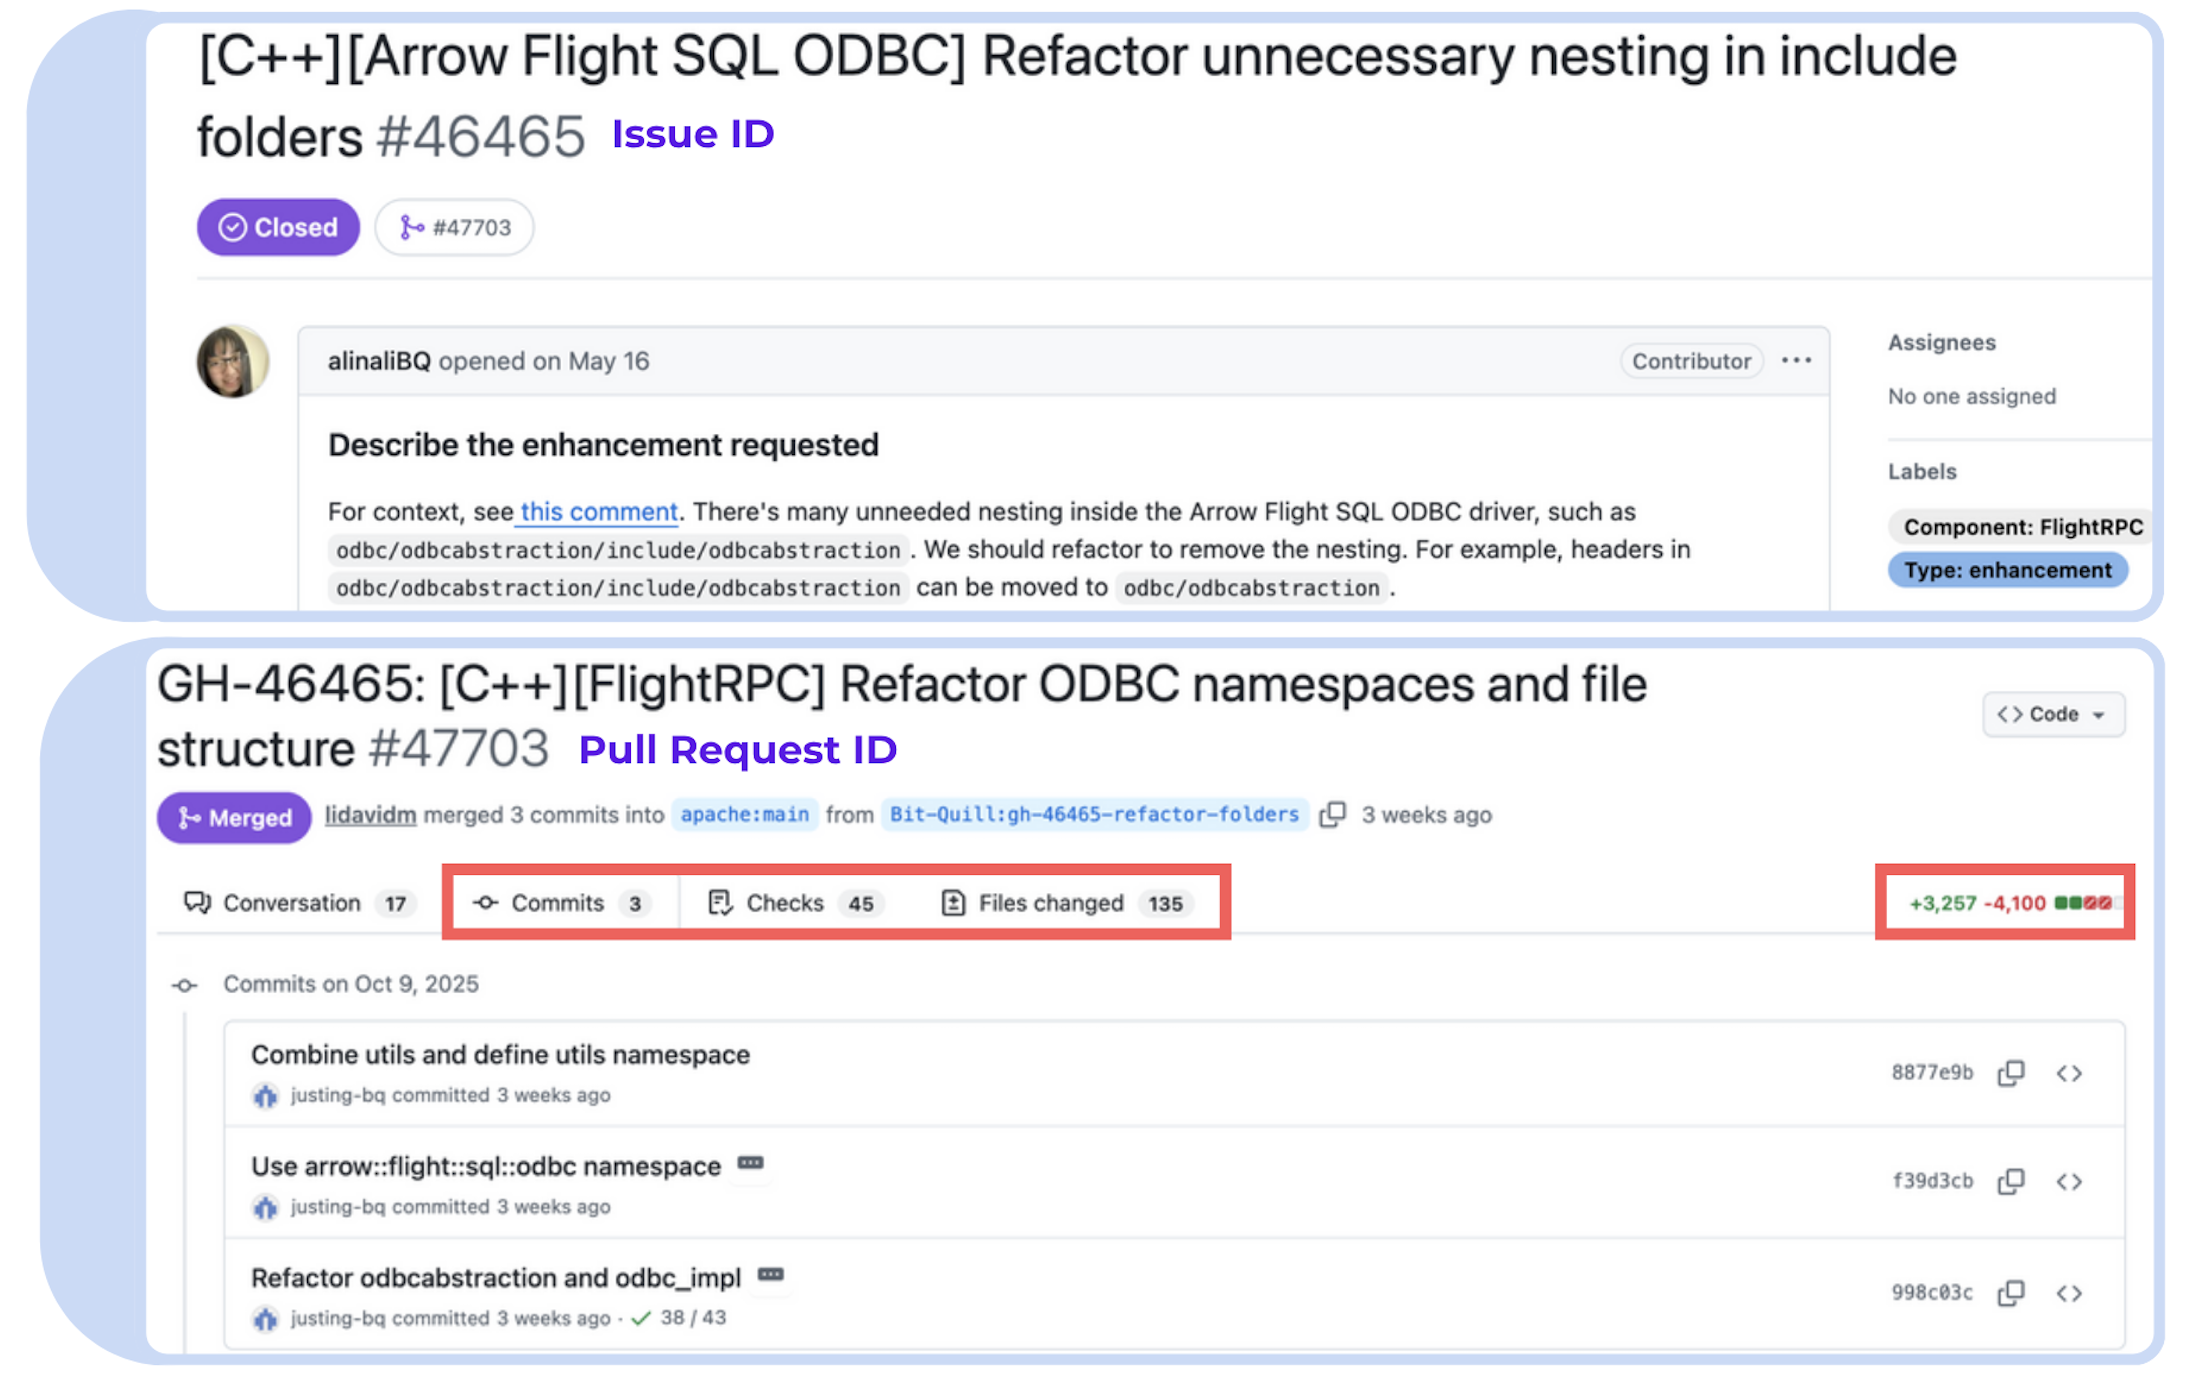
\includegraphics[width=0.9\textwidth]{Figures/issue-pr-demo-example.png}
        \captionsetup{font={small,it},justification=centering}
        \caption{A Practical Example of a One-to-Many Issue--Commit Relationship}
        \label{fig:issue_pr_demo_example}
    \end{figure}

\begin{enumerate}[a)]
	\item \textbf{Prevailing assumption: one-to-one issue--commit mappings.} Many automated methods are designed and evaluated under the assumption that each issue corresponds to a single commit. This simplifies modeling and evaluation but does not align with real development processes.
	
	\item \textbf{Prevalence of one-to-many relationships.} In practical development workflows a single issue, especially complex bugs or multi-step feature work, is often resolved through multiple commits (incremental fixes, follow-ups, or refactors)~\cite{r7,r17}. These one-to-many patterns are common in large and actively maintained projects. As shown in Fig.~\ref{fig:issue_pr_demo_example}, GitHub issue \texttt{\#46465}, titled \texttt{[C++] [Arrow Flight SQL ODBC] Refactor unnecessary nesting in include folders} was resolved by a series of three commits bundled in pull request \texttt{\#47703}. The commits (in order of time, earliest first) are:
    \begin{itemize}
        \setlength\itemsep{0pt}
        \setlength\parskip{0pt}
        \setlength\topsep{0pt}
        \item \textit{Commit 1: Refactor odbcabstraction and odbc\_impl}
        \item \textit{Commit 2: Use \texttt{arrow::flight::sql::odbc} namespace}
        \item \textit{Commit 3: Combine utils and define utils namespace}
        \end{itemize}

    The scope of this multi-step refactoring and its volume is shown by the \texttt{Files changed} tab, which indicates these three commits modified a total of 135 files, along with 3,257 lines of additions and 4,100 lines of deletions. This example illustrates the complexity of real-world issue resolution, where multiple coordinated commits are necessary to fully address a single issue.

	\item \textbf{Failure to capture full resolution scope.} By ignoring one-to-many links, current traceability models fail to capture the full history and context of issue resolution. This fragmentation degrades downstream tasks such as debugging, historical analysis, and automated repair, because the complete set of commits that together implement a fix is not recovered~\cite{r7}.
\end{enumerate}


\subsection{The business impact: high software maintenance costs}

Traceability gaps have direct operational consequences. When links between issues and their resolving commits are missing or incomplete, engineers spend extra time searching, re-running tests, and performing manual code reviews to determine what changed and why. This increases mean time to repair and contributes to ongoing maintenance expenses across large codebases~\cite{r15,r16}. For organizations operating at scale, the cumulative cost of these inefficiencies is non-trivial and motivates automated, accurate linking solutions.\\

\noindent
Together, these observations motivate a targeted focus on one-to-many issue–commit recovery. Solving this foundational problem produces immediate practical benefits for maintenance and research and provides a reliable substrate for higher-level agentic systems that aim to autonomously link, explain, and resolve software issues.

